
%% bare_jrnl.tex
%% V1.3
%% 2007/01/11
%% by Michael Shell
%% see http://www.michaelshell.org/
%% for current contact information.
%%
%% This is a skeleton file demonstrating the use of IEEEtran.cls
%% (requires IEEEtran.cls version 1.7 or later) with an IEEE journal paper.
%%
%% Support sites:
%% http://www.michaelshell.org/tex/ieeetran/
%% http://www.ctan.org/tex-archive/macros/latex/contrib/IEEEtran/
%% and
%% http://www.ieee.org/



% *** Authors should verify (and, if needed, correct) their LaTeX system  ***
% *** with the testflow diagnostic prior to trusting their LaTeX platform ***
% *** with production work. IEEE's font choices can trigger bugs that do  ***
% *** not appear when using other class files.                            ***
% The testflow support page is at:
% http://www.michaelshell.org/tex/testflow/


%%*************************************************************************
%% Legal Notice:
%% This code is offered as-is without any warranty either expressed or
%% implied; without even the implied warranty of MERCHANTABILITY or
%% FITNESS FOR A PARTICULAR PURPOSE! 
%% User assumes all risk.
%% In no event shall IEEE or any contributor to this code be liable for
%% any damages or losses, including, but not limited to, incidental,
%% consequential, or any other damages, resulting from the use or misuse
%% of any information contained here.
%%
%% All comments are the opinions of their respective authors and are not
%% necessarily endorsed by the IEEE.
%%
%% This work is distributed under the LaTeX Project Public License (LPPL)
%% ( http://www.latex-project.org/ ) version 1.3, and may be freely used,
%% distributed and modified. A copy of the LPPL, version 1.3, is included
%% in the base LaTeX documentation of all distributions of LaTeX released
%% 2003/12/01 or later.
%% Retain all contribution notices and credits.
%% ** Modified files should be clearly indicated as such, including  **
%% ** renaming them and changing author support contact information. **
%%
%% File list of work: IEEEtran.cls, IEEEtran_HOWTO.pdf, bare_adv.tex,
%%                    bare_conf.tex, bare_jrnl.tex, bare_jrnl_compsoc.tex
%%*************************************************************************

% Note that the a4paper option is mainly intended so that authors in
% countries using A4 can easily print to A4 and see how their papers will
% look in print - the typesetting of the document will not typically be
% affected with changes in paper size (but the bottom and side margins will).
% Use the testflow package mentioned above to verify correct handling of
% both paper sizes by the user's LaTeX system.
%
% Also note that the "draftcls" or "draftclsnofoot", not "draft", option
% should be used if it is desired that the figures are to be displayed in
% draft mode.
%

\documentclass[journal]{IEEEtran}
%
% If IEEEtran.cls has not been installed into the LaTeX system files,
% manually specify the path to it like:
% \documentclass[journal]{../sty/IEEEtran}

\usepackage{graphicx}
\usepackage{wrapfig}
\usepackage{cite}

% Some very useful LaTeX packages include:
% (uncomment the ones you want to load)


% *** MISC UTILITY PACKAGES ***
%
%\usepackage{ifpdf}
% Heiko Oberdiek's ifpdf.sty is very useful if you need conditional
% compilation based on whether the output is pdf or dvi.
% usage:
% \ifpdf
%   % pdf code
% \else
%   % dvi code
% \fi
% The latest version of ifpdf.sty can be obtained from:
% http://www.ctan.org/tex-archive/macros/latex/contrib/oberdiek/
% Also, note that IEEEtran.cls V1.7 and later provides a builtin
% \ifCLASSINFOpdf conditional that works the same way.
% When switching from latex to pdflatex and vice-versa, the compiler may
% have to be run twice to clear warning/error messages.






% *** CITATION PACKAGES ***
%
%\usepackage{cite}
% cite.sty was written by Donald Arseneau
% V1.6 and later of IEEEtran pre-defines the format of the cite.sty package
% \cite{} output to follow that of IEEE. Loading the cite package will
% result in citation numbers being automatically sorted and properly
% "compressed/ranged". e.g., [1], [9], [2], [7], [5], [6] without using
% cite.sty will become [1], [2], [5]--[7], [9] using cite.sty. cite.sty's
% \cite will automatically add leading space, if needed. Use cite.sty's
% noadjust option (cite.sty V3.8 and later) if you want to turn this off.
% cite.sty is already installed on most LaTeX systems. Be sure and use
% version 4.0 (2003-05-27) and later if using hyperref.sty. cite.sty does
% not currently provide for hyperlinked citations.
% The latest version can be obtained at:
% http://www.ctan.org/tex-archive/macros/latex/contrib/cite/
% The documentation is contained in the cite.sty file itself.






% *** GRAPHICS RELATED PACKAGES ***
%
\ifCLASSINFOpdf
  % \usepackage[pdftex]{graphicx}
  % declare the path(s) where your graphic files are
  % \graphicspath{{../pdf/}{../jpeg/}}
  % and their extensions so you won't have to specify these with
  % every instance of \includegraphics
  % \DeclareGraphicsExtensions{.pdf,.jpeg,.png}
\else
  % or other class option (dvipsone, dvipdf, if not using dvips). graphicx
  % will default to the driver specified in the system graphics.cfg if no
  % driver is specified.
  % \usepackage[dvips]{graphicx}
  % declare the path(s) where your graphic files are
  % \graphicspath{{../eps/}}
  % and their extensions so you won't have to specify these with
  % every instance of \includegraphics
  % \DeclareGraphicsExtensions{.eps}
\fi
% graphicx was written by David Carlisle and Sebastian Rahtz. It is
% required if you want graphics, photos, etc. graphicx.sty is already
% installed on most LaTeX systems. The latest version and documentation can
% be obtained at: 
% http://www.ctan.org/tex-archive/macros/latex/required/graphics/
% Another good source of documentation is "Using Imported Graphics in
% LaTeX2e" by Keith Reckdahl which can be found as epslatex.ps or
% epslatex.pdf at: http://www.ctan.org/tex-archive/info/
%
% latex, and pdflatex in dvi mode, support graphics in encapsulated
% postscript (.eps) format. pdflatex in pdf mode supports graphics
% in .pdf, .jpeg, .png and .mps (metapost) formats. Users should ensure
% that all non-photo figures use a vector format (.eps, .pdf, .mps) and
% not a bitmapped formats (.jpeg, .png). IEEE frowns on bitmapped formats
% which can result in "jaggedy"/blurry rendering of lines and letters as
% well as large increases in file sizes.
%
% You can find documentation about the pdfTeX application at:
% http://www.tug.org/applications/pdftex





% *** MATH PACKAGES ***
%
%\usepackage[cmex10]{amsmath}
% A popular package from the American Mathematical Society that provides
% many useful and powerful commands for dealing with mathematics. If using
% it, be sure to load this package with the cmex10 option to ensure that
% only type 1 fonts will utilized at all point sizes. Without this option,
% it is possible that some math symbols, particularly those within
% footnotes, will be rendered in bitmap form which will result in a
% document that can not be IEEE Xplore compliant!
%
% Also, note that the amsmath package sets \interdisplaylinepenalty to 10000
% thus preventing page breaks from occurring within multiline equations. Use:
%\interdisplaylinepenalty=2500
% after loading amsmath to restore such page breaks as IEEEtran.cls normally
% does. amsmath.sty is already installed on most LaTeX systems. The latest
% version and documentation can be obtained at:
% http://www.ctan.org/tex-archive/macros/latex/required/amslatex/math/





% *** SPECIALIZED LIST PACKAGES ***
%
%\usepackage{algorithmic}
% algorithmic.sty was written by Peter Williams and Rogerio Brito.
% This package provides an algorithmic environment fo describing algorithms.
% You can use the algorithmic environment in-text or within a figure
% environment to provide for a floating algorithm. Do NOT use the algorithm
% floating environment provided by algorithm.sty (by the same authors) or
% algorithm2e.sty (by Christophe Fiorio) as IEEE does not use dedicated
% algorithm float types and packages that provide these will not provide
% correct IEEE style captions. The latest version and documentation of
% algorithmic.sty can be obtained at:
% http://www.ctan.org/tex-archive/macros/latex/contrib/algorithms/
% There is also a support site at:
% http://algorithms.berlios.de/index.html
% Also of interest may be the (relatively newer and more customizable)
% algorithmicx.sty package by Szasz Janos:
% http://www.ctan.org/tex-archive/macros/latex/contrib/algorithmicx/




% *** ALIGNMENT PACKAGES ***
%
%\usepackage{array}
% Frank Mittelbach's and David Carlisle's array.sty patches and improves
% the standard LaTeX2e array and tabular environments to provide better
% appearance and additional user controls. As the default LaTeX2e table
% generation code is lacking to the point of almost being broken with
% respect to the quality of the end results, all users are strongly
% advised to use an enhanced (at the very least that provided by array.sty)
% set of table tools. array.sty is already installed on most systems. The
% latest version and documentation can be obtained at:
% http://www.ctan.org/tex-archive/macros/latex/required/tools/


%\usepackage{mdwmath}
%\usepackage{mdwtab}
% Also highly recommended is Mark Wooding's extremely powerful MDW tools,
% especially mdwmath.sty and mdwtab.sty which are used to format equations
% and tables, respectively. The MDWtools set is already installed on most
% LaTeX systems. The lastest version and documentation is available at:
% http://www.ctan.org/tex-archive/macros/latex/contrib/mdwtools/


% IEEEtran contains the IEEEeqnarray family of commands that can be used to
% generate multiline equations as well as matrices, tables, etc., of high
% quality.


%\usepackage{eqparbox}
% Also of notable interest is Scott Pakin's eqparbox package for creating
% (automatically sized) equal width boxes - aka "natural width parboxes".
% Available at:
% http://www.ctan.org/tex-archive/macros/latex/contrib/eqparbox/





% *** SUBFIGURE PACKAGES ***
%\usepackage[tight,footnotesize]{subfigure}
% subfigure.sty was written by Steven Douglas Cochran. This package makes it
% easy to put subfigures in your figures. e.g., "Figure 1a and 1b". For IEEE
% work, it is a good idea to load it with the tight package option to reduce
% the amount of white space around the subfigures. subfigure.sty is already
% installed on most LaTeX systems. The latest version and documentation can
% be obtained at:
% http://www.ctan.org/tex-archive/obsolete/macros/latex/contrib/subfigure/
% subfigure.sty has been superceeded by subfig.sty.



%\usepackage[caption=false]{caption}
%\usepackage[font=footnotesize]{subfig}
% subfig.sty, also written by Steven Douglas Cochran, is the modern
% replacement for subfigure.sty. However, subfig.sty requires and
% automatically loads Axel Sommerfeldt's caption.sty which will override
% IEEEtran.cls handling of captions and this will result in nonIEEE style
% figure/table captions. To prevent this problem, be sure and preload
% caption.sty with its "caption=false" package option. This is will preserve
% IEEEtran.cls handing of captions. Version 1.3 (2005/06/28) and later 
% (recommended due to many improvements over 1.2) of subfig.sty supports
% the caption=false option directly:
%\usepackage[caption=false,font=footnotesize]{subfig}
%
% The latest version and documentation can be obtained at:
% http://www.ctan.org/tex-archive/macros/latex/contrib/subfig/
% The latest version and documentation of caption.sty can be obtained at:
% http://www.ctan.org/tex-archive/macros/latex/contrib/caption/




% *** FLOAT PACKAGES ***
%
%\usepackage{fixltx2e}
% fixltx2e, the successor to the earlier fix2col.sty, was written by
% Frank Mittelbach and David Carlisle. This package corrects a few problems
% in the LaTeX2e kernel, the most notable of which is that in current
% LaTeX2e releases, the ordering of single and double column floats is not
% guaranteed to be preserved. Thus, an unpatched LaTeX2e can allow a
% single column figure to be placed prior to an earlier double column
% figure. The latest version and documentation can be found at:
% http://www.ctan.org/tex-archive/macros/latex/base/



%\usepackage{stfloats}
% stfloats.sty was written by Sigitas Tolusis. This package gives LaTeX2e
% the ability to do double column floats at the bottom of the page as well
% as the top. (e.g., "\begin{figure*}[!b]" is not normally possible in
% LaTeX2e). It also provides a command:
%\fnbelowfloat
% to enable the placement of footnotes below bottom floats (the standard
% LaTeX2e kernel puts them above bottom floats). This is an invasive package
% which rewrites many portions of the LaTeX2e float routines. It may not work
% with other packages that modify the LaTeX2e float routines. The latest
% version and documentation can be obtained at:
% http://www.ctan.org/tex-archive/macros/latex/contrib/sttools/
% Documentation is contained in the stfloats.sty comments as well as in the
% presfull.pdf file. Do not use the stfloats baselinefloat ability as IEEE
% does not allow \baselineskip to stretch. Authors submitting work to the
% IEEE should note that IEEE rarely uses double column equations and
% that authors should try to avoid such use. Do not be tempted to use the
% cuted.sty or midfloat.sty packages (also by Sigitas Tolusis) as IEEE does
% not format its papers in such ways.


%\ifCLASSOPTIONcaptionsoff
%  \usepackage[nomarkers]{endfloat}
% \let\MYoriglatexcaption\caption
% \renewcommand{\caption}[2][\relax]{\MYoriglatexcaption[#2]{#2}}
%\fi
% endfloat.sty was written by James Darrell McCauley and Jeff Goldberg.
% This package may be useful when used in conjunction with IEEEtran.cls'
% captionsoff option. Some IEEE journals/societies require that submissions
% have lists of figures/tables at the end of the paper and that
% figures/tables without any captions are placed on a page by themselves at
% the end of the document. If needed, the draftcls IEEEtran class option or
% \CLASSINPUTbaselinestretch interface can be used to increase the line
% spacing as well. Be sure and use the nomarkers option of endfloat to
% prevent endfloat from "marking" where the figures would have been placed
% in the text. The two hack lines of code above are a slight modification of
% that suggested by in the endfloat docs (section 8.3.1) to ensure that
% the full captions always appear in the list of figures/tables - even if
% the user used the short optional argument of \caption[]{}.
% IEEE papers do not typically make use of \caption[]'s optional argument,
% so this should not be an issue. A similar trick can be used to disable
% captions of packages such as subfig.sty that lack options to turn off
% the subcaptions:
% For subfig.sty:
% \let\MYorigsubfloat\subfloat
% \renewcommand{\subfloat}[2][\relax]{\MYorigsubfloat[]{#2}}
% For subfigure.sty:
% \let\MYorigsubfigure\subfigure
% \renewcommand{\subfigure}[2][\relax]{\MYorigsubfigure[]{#2}}
% However, the above trick will not work if both optional arguments of
% the \subfloat/subfig command are used. Furthermore, there needs to be a
% description of each subfigure *somewhere* and endfloat does not add
% subfigure captions to its list of figures. Thus, the best approach is to
% avoid the use of subfigure captions (many IEEE journals avoid them anyway)
% and instead reference/explain all the subfigures within the main caption.
% The latest version of endfloat.sty and its documentation can obtained at:
% http://www.ctan.org/tex-archive/macros/latex/contrib/endfloat/
%
% The IEEEtran \ifCLASSOPTIONcaptionsoff conditional can also be used
% later in the document, say, to conditionally put the References on a 
% page by themselves.





% *** PDF, URL AND HYPERLINK PACKAGES ***
%
%\usepackage{url}
% url.sty was written by Donald Arseneau. It provides better support for
% handling and breaking URLs. url.sty is already installed on most LaTeX
% systems. The latest version can be obtained at:
% http://www.ctan.org/tex-archive/macros/latex/contrib/misc/
% Read the url.sty source comments for usage information. Basically,
% \url{my_url_here}.





% *** Do not adjust lengths that control margins, column widths, etc. ***
% *** Do not use packages that alter fonts (such as pslatex).         ***
% There should be no need to do such things with IEEEtran.cls V1.6 and later.
% (Unless specifically asked to do so by the journal or conference you plan
% to submit to, of course. )


% correct bad hyphenation here
\hyphenation{op-tical net-works semi-conduc-tor}


\begin{document}
%
% paper title
% can use linebreaks \\ within to get better formatting as desired
\title{SAME: An Extended Semantic-Aware Multi-tiered Source Deduplication Framework on Cloud Backup}
%
%
% author names and IEEE memberships
% note positions of commas and nonbreaking spaces ( ~ ) LaTeX will not break
% a structure at a ~ so this keeps an author's name from being broken across
% two lines.
% use \thanks{} to gain access to the first footnote area
% a separate \thanks must be used for each paragraph as LaTeX2e's \thanks
% was not built to handle multiple paragraphs
%

\author{{Chynna~Julia~Cordevilla, Rafael~Gerard~Formes, Francis~Bien~Jan~Viernes}% <-this % stops a space
}

% note the % following the last \IEEEmembership and also \thanks - 
% these prevent an unwanted space from occurring between the last author name
% and the end of the author line. i.e., if you had this:
% 
% \author{....lastname \thanks{...} \thanks{...} }
%                     ^------------^------------^----Do not want these spaces!
%
% a space would be appended to the last name and could cause every name on that
% line to be shifted left slightly. This is one of those "LaTeX things". For
% instance, "\textbf{A} \textbf{B}" will typeset as "A B" not "AB". To get
% "AB" then you have to do: "\textbf{A}\textbf{B}"
% \thanks is no different in this regard, so shield the last } of each \thanks
% that ends a line with a % and do not let a space in before the next \thanks.
% Spaces after \IEEEmembership other than the last one are OK (and needed) as
% you are supposed to have spaces between the names. For what it is worth,
% this is a minor point as most people would not even notice if the said evil
% space somehow managed to creep in.



% The paper headers
\markboth{Networks and Distributed Systems Group, 2013-2014}%
{Viernes \MakeLowercase{\textit{et al.}}: Numerical Analysis of Transient Charge Partitioning}
% The only time the second header will appear is for the odd numbered pages
% after the title page when using the twoside option.
% 
% *** Note that you probably will NOT want to include the author's ***
% *** name in the headers of peer review papers.                   ***
% You can use \ifCLASSOPTIONpeerreview for conditional compilation here if
% you desire.




% If you want to put a publisher's ID mark on the page you can do it like
% this:
%\IEEEpubid{0000--0000/00\$00.00~\copyright~2007 IEEE}
% Remember, if you use this you must call \IEEEpubidadjcol in the second
% column for its text to clear the IEEEpubid mark.



% use for special paper notices
%\IEEEspecialpapernotice{(Invited Paper)}




% make the title area
\maketitle


\begin{abstract}
%\boldmath
Goes here
\end{abstract}
% IEEEtran.cls defaults to using nonbold math in the Abstract.
% This preserves the distinction between vectors and scalars. However,
% if the journal you are submitting to favors bold math in the abstract,
% then you can use LaTeX's standard command \boldmath at the very start
% of the abstract to achieve this. Many IEEE journals frown on math
% in the abstract anyway.

% Note that keywords are not normally used for peerreview papers.
%\begin{IEEEkeywords}
%IEEEtran, journal, \LaTeX, paper, template.
%\end{IEEEkeywords}






% For peer review papers, you can put extra information on the cover
% page as needed:
% \ifCLASSOPTIONpeerreview
% \begin{center} \bfseries EDICS Category: 3-BBND \end{center}
% \fi
%
% For peerreview papers, this IEEEtran command inserts a page break and
% creates the second title. It will be ignored for other modes.
\IEEEpeerreviewmaketitle



\section{Introduction}
% The very first letter is a 2 line initial drop letter followed
% by the rest of the first word in caps.
% 
% form to use if the first word consists of a single letter:
% \IEEEPARstart{A}{demo} file is ....
% 
% form to use if you need the single drop letter followed by
% normal text (unknown if ever used by IEEE):
% \IEEEPARstart{A}{}demo file is ....
% 
% Some journals put the first two words in caps:
% \IEEEPARstart{T}{his demo} file is ....
% 
% Here we have the typical use of a "T" for an initial drop letter
% and "HIS" in caps to complete the first word.
\IEEEPARstart{C}{loud} computing is catching on fast, and people are becoming more and more reliant on storing and processing their data on the cloud. In fact, in today’s world, the explosion in the volume of online digital content resulted in an enormous strain on storage systems. According to the recent study of the International Data Corporation, 2.8 Zettabytes of data will have been created and replicated in 2012. By 2020, it is predicted that the digital universe will skyrocket to 40 ZB, an amount that exceeds previous forecasts. As cloud computing’s role grows in the management of the Big Data, the number of servers worldwide is expected to grow tenfold and the amount of information managed directly by enterprise data centers will grow by a factor of 14. [1] The digital universe lives increasingly in a computing cloud, above terra firma of vast hardware data centers linked to billions of distributed devices. The continuous barrage of data (the addition, deletion, and updating of data) on cloud servers creates a problem that database designers are familiar with: data duplication, or the presence of data duplicates.

Data duplication is a problem, most especially in the cloud, for the following reasons:

\begin{enumerate}
	\item Wasted storage space; redundant storage means more storage space is used up. This is going to be a problem if the space being used or allotted for various users is/are limited.

	\item Data inconsistency; it is highly likely that a file update will get lost among the redundant data, because various links still point to all the previous version/s of said file. This is a huge problem most especially if the cloud server is shared among different users.

	\item Slow data searches and high data management costs; redundant storage would mean that the system would have to go through a lot more data than it should to be able to find a single file. This is going to be a huge problem if the cloud holds a lot of data. 

	\item Slow data transmission; having duplicates in a system would mean more backups, and a longer wait for data to transmit.
\end{enumerate}

These are why data duplication must be addressed, and data deduplication (as the name implies), does exactly that. 

\subsection{Significance of Study}

Many deduplication services have sprouted through the years as storage systems have evolved into a necessity for business and personal use alike. All these aim to solve the problems aforementioned, making the storage process more efficient than it would without deduplication.

Research on the use of deduplication methods that efficiently reduce space occupied by redundant data have already been done, beginning with simple storage systems [12] and with how data can be stored in a manner that would make it easier for future computations such as data access and retrieval [5], making its way into data streams [8], even to adding interfaces to mediate data transmissions [7], and finally, into cloud storage systems [1][2], cloud backup systems [3][4], that involve mobile systems [9] as well.

However, despite being a solution, researchers have proven that deduplication holds much room for improvement. Many researchers have been working on ways to improve the deduplication process, looking into various hashing techniques, applying various algorithms, and rearranging the architectures of their systems with the goal to optimize them further.

One such improvement we are interested in is the application of semantic-awareness into the deduplication system.

\subsection{Scope, Limitations, and Objectives of the Study}

Among the numerous applications of data deduplication, this study aims to focus on Cloud Backup due to the reason that Cloud Storage is a booming industry and innovations within this field will be helpful towards advancing said technology. There is also much room for improvement and study within this field, as the architecture is quite different from older systems.

Initially, we wanted to delve into the manipulation of semantic data for efficiency, as the use of semantic and contextual data has proven very useful to recent studies and projects. The Semantic Aware Multi-Tiered Source Deduplication Framework is a notable deduplication solution that uses file semantics (e.g. file locality, file type, file size, file timestamps), and it aims to achieve an optimal tradeoff between deduplication efficiency and deduplication overhead. We decided that its use of file semantics, its application to Cloud Backup and Cloud Storage, and its achieved ratio between efficiency and overhead makes it an appropriate framework to study and add on to. Hence, we develop SAMe: an Extended Semantic Aware Multi-Tiered Source Deduplication Framework for Cloud Backup.

Having already given the scope, the objectives of SAMe are as follows:
\begin{enumerate}
\item[$\bullet$]To readily solve the aforementioned duplication problems: wasted storage space, data inconsistency, slow data searches, and slow data transmission.
\item[$\bullet$]To improve the deduplication solution the SAM offers by adding additional semantics.
\item[$\bullet$]To significantly reduce deduplication overhead, deduplication time, disk IO, and the bandwidth eaten up by deduplication.
\end{enumerate}

The following sections of this paper is organized as follows. Section II will contain a review of literature related to our study, giving reasons as to why the solutions present in SAM are viable and efficient, and why our additional semantics are viable and efficient, as well. We placed our methodology in Section III, wherein we describe the specifics of the algorithms we used, test data, and other important data we used throughout the duration of experimenting and testing. In Section IV we further discuss our attained results.

\section{Review of Related Literature}

\subsection{Data Deduplication}

Data Deduplication is a specialized data compression technique for removing duplicate copies of repeated data. Deduplication is considered to be the most important emerging technology in the field of data storage backup research [14]. Most deduplication research focuses on the improvement of each step of its major processes, namely: data storage, data partitioning, indexing, and searching.

Existing deduplication solutions make use of various methods to make data deduplication faster and more efficient. Some known solutions make use of compression in the chunk-level and/or file-level, global and/or local deduplication [4], hashing [1] and, recently, the exploitation of file semantics [4][12][13]. This section will focus on the general considerations made when creating a deduplication system.

\subsubsection{Data Storage and Partitioning}

\paragraph{File-level vs. Chunk-level}

The speed and efficiency of the data deduplication process is heavily-reliant on how the data is represented and partitioned in the system, therefore numerous research has been done with regard to this topic. Two types of data partitioning have been implemented in these research, namely: a) saving data as files, and b) partitioning data into chunks. It is important to take note that speed and accuracy are factors that should be considered when determining which type will best serve the deduplication process one has in mind. Focusing on the chunk-level has been proven accurate for data deduplication, but at the cost of more lookups which demands more memory for computations. This is slower compared to focusing on the file-level which has fewer lookups, since the chunk-level has more elements that should be compared to each other. Searching within the file-level, however, is less accurate when it comes to duplicate detection.

Regarding data chunking, data used to be divided into meaningless chunks with fixed sizes until projects such as Semantic Data Deduplication (SDD) [12] came about and used file semantics in the process of chunk-partitioning, since the researchers behind SDD believed that grouping data by factors that they have in common will make the searching process faster. SDD proved to be able to reduce the storage used by 20-50 percent compared to methods preceding it. Data-writing performance also increased by 50-70 percent.

\paragraph{Local vs. Global}

In addition to the types of data-partitioning, there is also another factor to be considered in deduplication, and that is: the scope of the deduplication. Deduplication can be applied locally, or within the client’s filesystem. This means only having to go through files or chunks that are stored within a single computer. Deduplication can also be applied on a global level, where the process would look into either files or chunks across clients and across servers to check each for duplicates. 

Recent research use hybrids of both global and local, file-level and chunk-level deduplication. 

One such example is the AA-Dedupe [4], which is a deduplicating application that caters to four factors (i.e. a large percentage of storage is occupied by a very small number of large files with very low sub-file redundancy) surveyed in an experiment. The application adapts to these scenarios and switches to chunk or file level, whichever is best for the situation.

SAM [3], on the other hand, uses a hybrid of both chunk-level and file-level approaches. SAM makes use of chunk-level deduplication locally, while using file-level deduplication for a broader, global level, e.g. for comparing and for searching across multiple computers. Using chunks in the global level would mean longer searches, and using files on the local level would mean lesser accuracy, hence, SAM’s idea of using both chunk-level and file-level approaches within their proper areas achieves greater speed and efficiency. In fact, one of the main goals of this particular research is to “achieve an optimal tradeoff between deduplication efficiency and deduplication overhead to maintain a shorter backup window than existing solutions“, which it has proven to do in the end.

\paragraph{Scope vs. Target}

Aside from considering both the data-partitioning and the scope of deduplication, a third factor exists: the area upon which deduplication must be applied. 

There are two classifications under this factor: a) source deduplication, and b) target deduplication. Source deduplication removes redundant data before any transmission occurs. This helps reduce the bandwidth used for transmission. Target deduplication, on the other hand, removes redundant data as the data is transmitted, e.g. between the source and backup target. Unlike with source deduplication, target deduplication does not help with reducing the bandwidth. Target deduplication, however, is a better option for larger sets of data, although it requires some hardware to be placed at remote sites.
\\
\subsubsection{Indexing and Searching Methods}
\\
Determining which indexing and searching methods should be used is very essential to the speed and efficiency of the entire deduplication process, as these functions are what run during the entire procedure.

Hashing is used in deduplication, as it provides a quick solution to data accessing. The ones most frequently used in deduplication are both MD5 and SHA-1, since these algorithms are the least likely to garner hash collisions (MD5 with the hash collision probability of $\frac{1}{2^{28}}$ and SHA-1 with $\frac{1}{2^{160}}$, which is important in deduplication, since file-uniqueness is being tested.

Since hashing is to be applied in deduplication, it becomes an additional factor to be considered when choosing how to store files (chunk vs. file) and when deduplication must be used (global vs. local).

In an experiment worth 475.2 GB of data, the deduplication size they computed was 37GB, but the final size was 38.1GB. The extra 1.1GB came from the extra data created from lookups, which is still good. This goes to show that storage isn’t the only factor to be focused on when it comes to deduplication, but also efficiency on reads and writes, file integrity, and the like, and the use of good hashing and indexing techniques make such efficiencies possible.

\subsubsection{Applications and Testing}

Deduplication would be useless without any applications to use it with. Most studies on deduplication deals with testing the efficiency of their deduplication process using their own unique applications. The niches covered range from applying deduplication in Virtual Machine clouds [11][14] to creating a deduplicating language known as Dedupalog [13]. Other applications involve applying deduplication methods onto platforms such as the Mobile Web [9].

\subsection{The Semantic-Aware Multi-Tiered Source De-duplication Framework for Cloud Backup (SAM)}

\subsubsection{Semantic-Aware Systems with Data Deduplication}

\subsubsection{SAM Baselines}

Two well-known and widely-used methods of deduplication are the Local Chunk Deduplication Scheme (L-CDS), which chunks files locally (leaving 40.69 percent of redundant data), and the Global Chunk Deduplication Scheme (G-CDS), which chunks files on a global scale (leaving 0 percent redundant data). Despite being extremely efficient in deduplicating, however, G-CDS leaves much room for improvement in deduplication overhead. Both baselines have been used by SAM for it to achieve its goal of achieving an optimal tradeoff between efficiency and overhead.

\subsubsection{SAM Semantics}

Studies have shown that similar and/or related data are likely to have unneeded file duplicates, proving that the use of file semantics as a factor could greatly improve the deduplication process.

One of the earliest examples of such research is [12], which uses semantic information such as Application Metadata (file type, file format), Application or User Tags (blog tags, multimedia tags), and Filesystem Metadata, to be able to chunk all related data together into what the researchers call “Semantic Chunks” or SCs. The system then obtains these SCs and stores them further into fixed-sized objects for easier data management, which are then stored in Intelligent Storage Nodes or ISNs for quick searching. The method proposed in [12] reduces the used storage by 20-50 percent compared to methods before it. Data-writing performance also increases by 50-70 percent.

SAM follows this trend and is noteworthy because of its clever utilization and addition of file semantics to effective methods of deduplication. “Many file-semantics attributes can be exploited to narrow down the search space of redundant data, which can reduce the overall deduplication overhead while maintaining high deduplication efficiency.” [3] SAM utilized this fact to drastically reduce Disk IO, hence, decreasing time and overhead as well. 

“File semantics can be revealed at various levels, including definitional, associative, structural, environmental level or through other relative information of the files, where various hints can be obtained.” [3] SAM focuses on File Locality, File Size, File Type, and File Timestamp.

\begin{itemize}
	\item \textbf{File Locality.} SAM uses this semantic hand-in-hand with caching. Studies say that it is likely that the files in a folder with a duplicate file are also duplicates of other files found within the folder where the original file resides. With that being said, SAM caches files that have the same locality as previously checked original files so that searching is made more efficiently.

	\item \textbf{File Size.} SAM had concluded that files that are less than 8KB are to be ignored due to their research. It is said that 63.8 percent of the files in the storage are less than or equal to the said size. These files are checked and they deduced that these small files have only 0.53 percent chances of getting duplicated, plus it reduces the overhead of the process.

	\item \textbf{File Type.} When it comes to chunking, SAM filters out multimedia files and compressed files, as these files are represented differently in binary form, thus, updates aren’t detected via chunking. Also, multimedia files are less likely to be updated, and are the least likely to have similarities in chunks that will determine overall similarity, so SAM usually leaves these types solely to file deduplication.
	
	\item \textbf{File Timestamp.} SAM also exploits the file timestamps to easily determine what files could possibly be updated / changed. A file is unchanged simply if the timestamp is also unchanged, removing it from the deduplication process, lowering the lookups.
	
\end{itemize}

\subsubsection{SAM Phases}

\begin{figure}[!t]
\centering
\includegraphics[height=2.5in, width=3.5in]{image6.png}
\caption{SAM Phases}
\end{figure}

SAM’s architecture consists of three parts: the File Agent, the Master Server, and the Storage Server. The File Agent resides in each client computer, and is in charge of all local processes to do with the client’s filesystem. Such processes include file hashing, sending file hash lists to the Master Server, chunking files, and sending chunks to the Storage Server. The Master Server, on the other hand, is in charge of gathering lists of file hashes from different clients and checking them for duplicates. Only lists are stored in the Master Server, as all its processing power is used for comparison and indexing. The Storage Server is where all the file chunks are stored and backed up.

Having each part’s main goals arranged linearly in order, SAM’s entire system can be arranged into three phases: Virtual Full Backup (VFB), Global File-level Deduplication (GFD), Local Chunk-level Deduplication (LCD), all of which will be discussed in the methodology section of this paper.

\section{Methodology}

We used SAM as our baseline and from there, we would compare our work, from optimizations to different/additional algorithms.

\subsection{Implementation of SAM}

There are 3 major stages that divides the whole SAM process. And these are the following:

\begin{enumerate}
\item \textbf{Virtual Full Backup}: This is the initial filter of duplicates. Files are checked locally within each of the clients where they would send the only ones that are unique. Each files are checked through its attributes and hashes to help determine more easily if the file is changed or not.
After checking, they are then hashed and are sent the master server.
\item \textbf{Global File-Level Deduplication}: The sent hashes, from all of its clients, are received by the master server and are then to be further filtered. If there are duplicate files with the other clients, they are then notified back to the clients to not send that/those specific file/s. Multimedia files won’t be checked anymore, immediately chunking it and sending directly to the master server; this is because a change to a single pixel (multimedia, for example .jpeg file) would give a very different hash. After these, the clients will now proceed to chunking.
\item \textbf{Local Chunk-Level Deduplication}: The clients will now chunk the files that are labeled unique by the master server and will send these chunks to the storage server to be saved.
\end{enumerate}

\subsection{Operating System}
We used Ubuntu 14.01 as the environment where we ran the baseline. Soon, we would be porting part of our code to Windows 8 to build the software for the client’s side; the server side code will still be ran in Ubuntu. This is because we initially planned this program for Microsoft Windows users, and soon, would also open up to the other common operating systems.

\subsection{Dataset}
The dataset that we first used were .txt, .png, .jpg, .doc, .ppt, .mp3, .html, .scl and .c to give an approximate to the files that a student usually saves via cloud. We got samples of these files of roughly 2.4GB worth of unique files and distributed them randomly, with repetitions, to a certain number of folders (our temporary “clients”) resulting to 11.46GB of files to be tested (Fig 4). We created the datasets we used such that they mirror how real-world student filesystems look like, adding mostly study material and organizing them in ways as how we would likewise organize them.

\subsection{Assessment}
\subsubsection{Total percentage of duplicates}
For our initial testing, we pre-determined the size (2.4GB as stated previously) then we randomly distribute those files throughout different folders and determine the whole size. The percentage of the size of duplicates would be determined by the excess size from the 2.4GB.

\begin{figure}[!t]
\centering
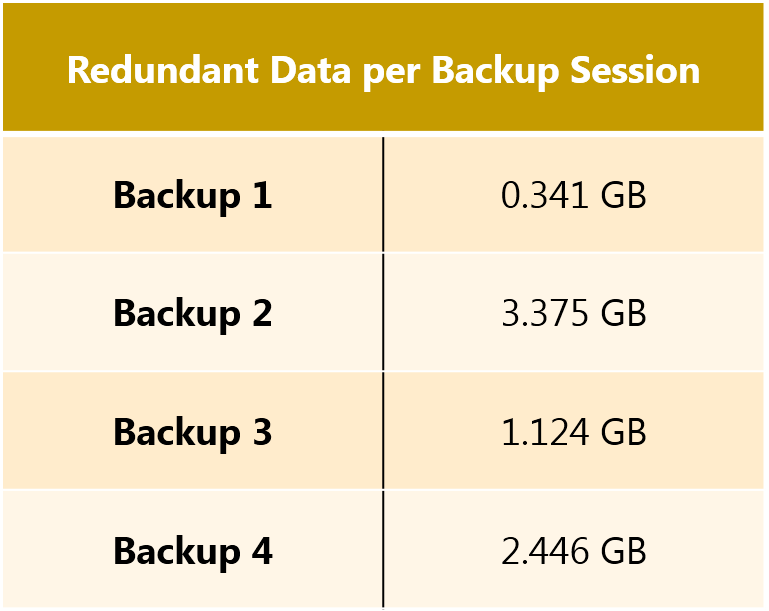
\includegraphics[height=1.5in, width=2in]{image1.png}
\caption{Redundant data per session.}
\end{figure}

\begin{figure}[!t]
\centering
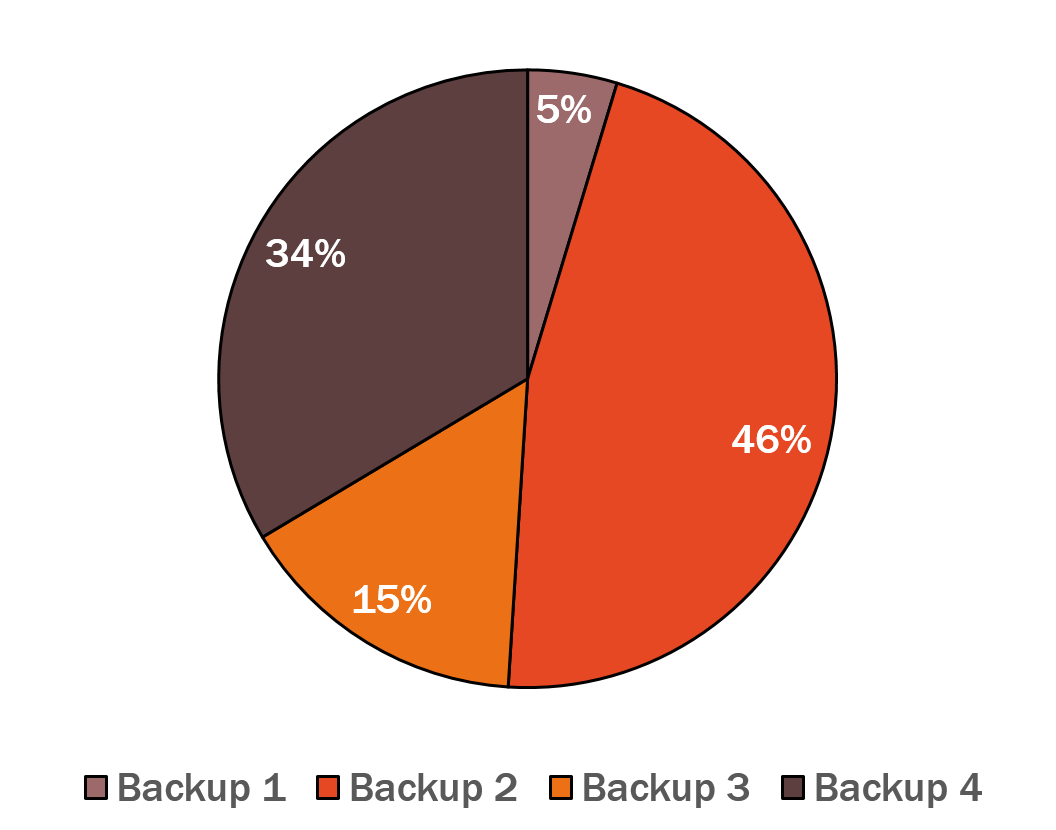
\includegraphics[height=2in, width=3in]{image3.png}
\caption{Redundant data per session (in percentage).}
\end{figure}

\subsubsection{Deduplication Efficiency}
\begin{itemize}
\item \textbf{Time and Memory}. Time efficiency would be determined based on the baseline which is SAM[3]. If the length of the process is comparable to the baseline (or even better, which is our target), then we can say that it is acceptable enough. But another thing that should be considered is the amount of memory or lookups it takes up. There should be a trade-off between the both and that will be cleared off during the tests and runs.
\item \textbf{Size and integrity}. Efficiency would also be determined by its resulting size. Since the size of our unique files would be 2.4GB, then the resulting size of the 11.46GB test data must also be 2.4GB; that is if the deduplication is dependent on file comparison. Since we are deduplicating files at the chunk level, we may see results that are of size 2.4GB (for this test data) or even less, depending on how many duplicate chunks we can find. Of course the chunks must be tested if they can be reverted back to its full file form to confirm its consistency and integrity.
\end{itemize}

\subsubsection{Deduplication Overhead}
Deduplication overhead is described in terms of latency and reduced throughput. This would depend on how fast the server reacts to the clients and vice versa; also, data exchange from both sides should be successful and should avoid any penalties (packet losses, delays, etc.).

\subsubsection{Backup Window}
The backup window represents the time spent sending a particular dataset to a backup destination. The backup window consists of two parts: data de-duplication time and data transfer time. To obtain a fixed dataset, the de-duplication time is generally fixed, whereas the data transfer time varies with network bandwidth.

\subsubsection{Future Work}
A good suggestion for future work regarding this project would be to create larger datasets, for a more thorough and accurate testing of our system. Perhaps, to obtain a few real-world datasets from willing participants will be sufficient. Related to testing, the frequency of each “wave” or each “run” of the program must also be considered in order to get a more accurate understanding of the system’s backup window. 

On a more methodological level, to add additional file semantics that would help boost deduplication efficiency and reduce overhead is another good thing to be added. Such a semantic that can be used is File Age. Delta Encoding can also be added for version control. 

Another improvement that can be applied is to be able to port this system to various other platforms (Linux and Mac OS for the File Agent, Windows and Mac OS for the servers).


\section{Results and Discussion}

We have created a simulator for SAM and fed the preliminary dataset specified in the previous section to evaluate SAM'S performance.

Given the percentage of duplicates as seen in figure 5, we managed to generate results (fig 6)  that gives us SAM's average dedup efficiency of 94.8375 percent, which leaves about 5.1625 percent of redundancy intact. As one can see in fig 7 and fig 8, SAM's results are very close to 100 percent efficiency.

We ran our application and we got results that were slightly comparable to SAM, but what we didn’t account for yet was the time it took for the whole process. We tried to see first if our deduplication process, at its basic form, would give considerable results.

We've also simulated the data transmission of the to-be-backed-up files using varying bandwidth and transmission speed (fig 9). Again, the results that we have obtained are almost similar to SAM's, the difference accounts to the diversity of the original paper's dataset.

\begin{figure}[!t]
\centering
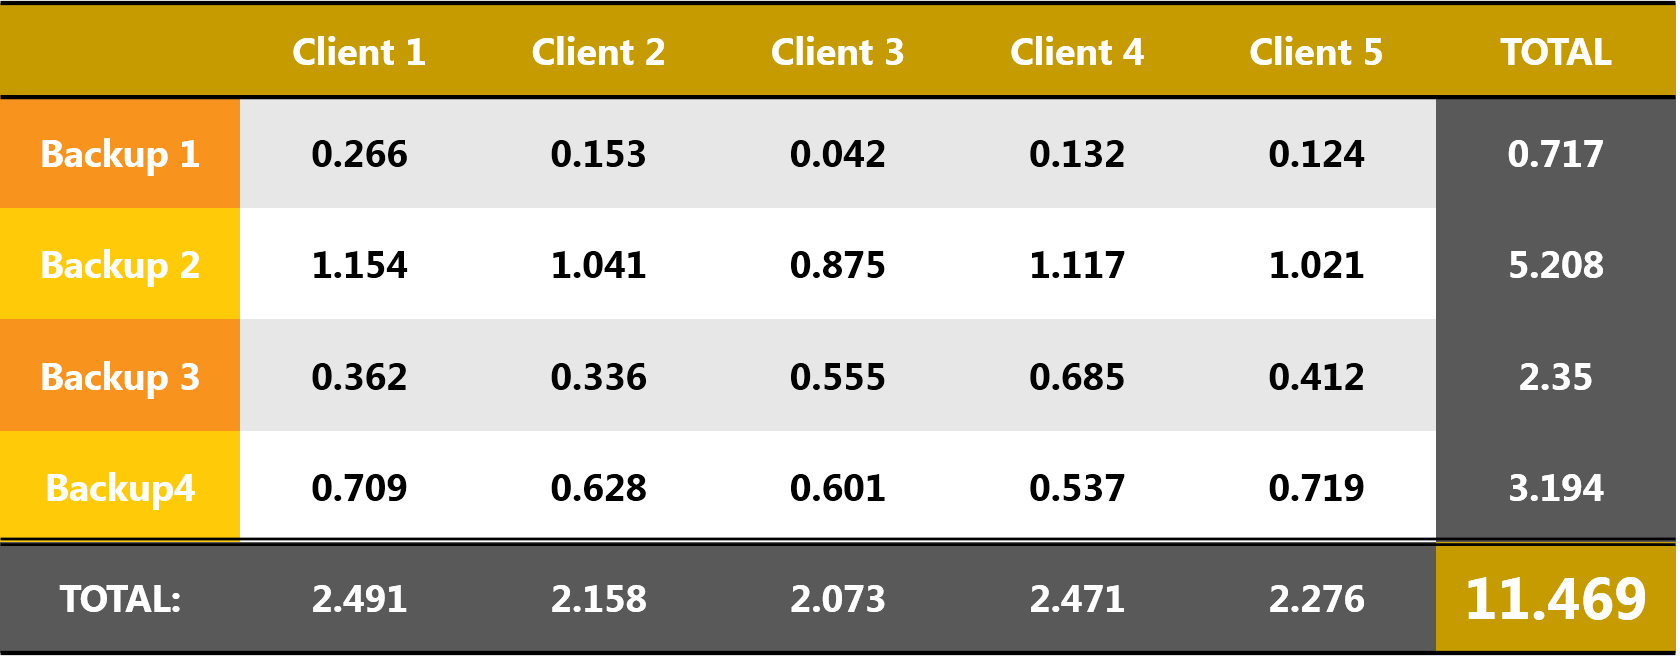
\includegraphics[height=1.5in, width=3in]{image2.png}
\caption{Dataset across five clients in four backup sessions. All numbers are in Gb.}
\end{figure}

\begin{figure}[!t]
\centering
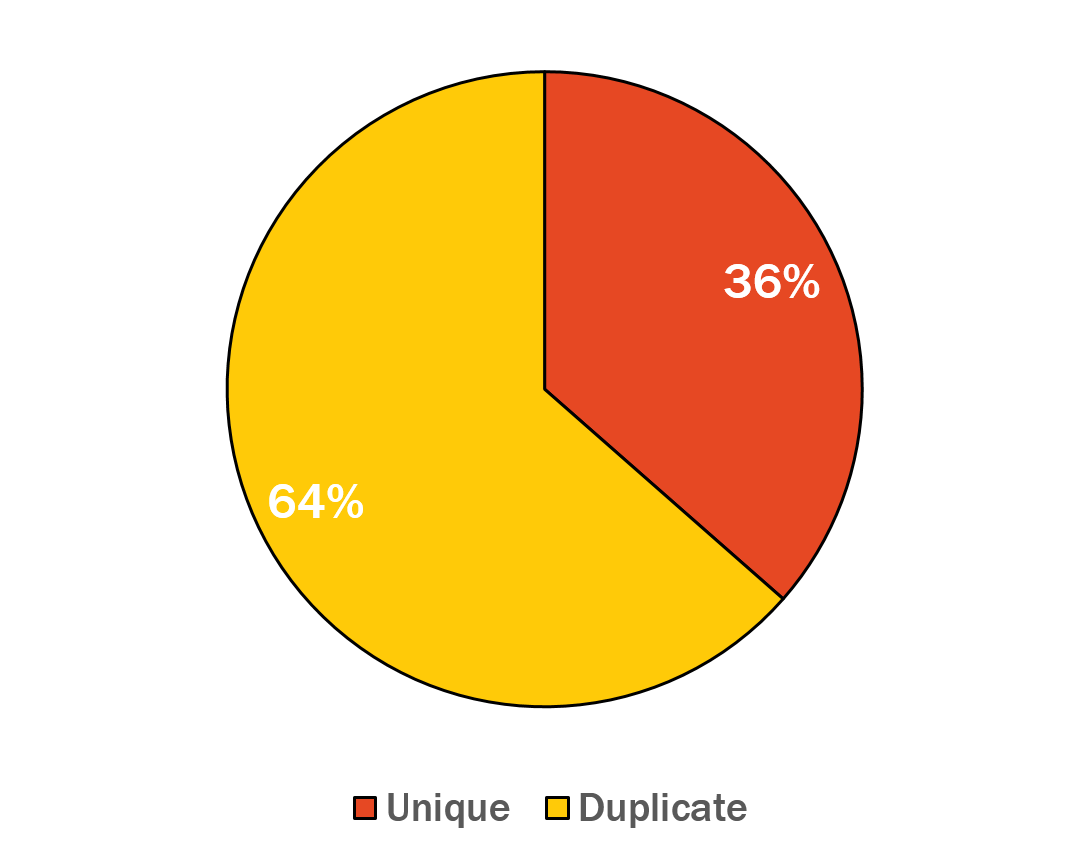
\includegraphics[height=2in, width=3in]{image4.png}
\caption{Unique vs duplicated data in percentage in our dataset.}
\end{figure}

\begin{figure}[!t]
\centering
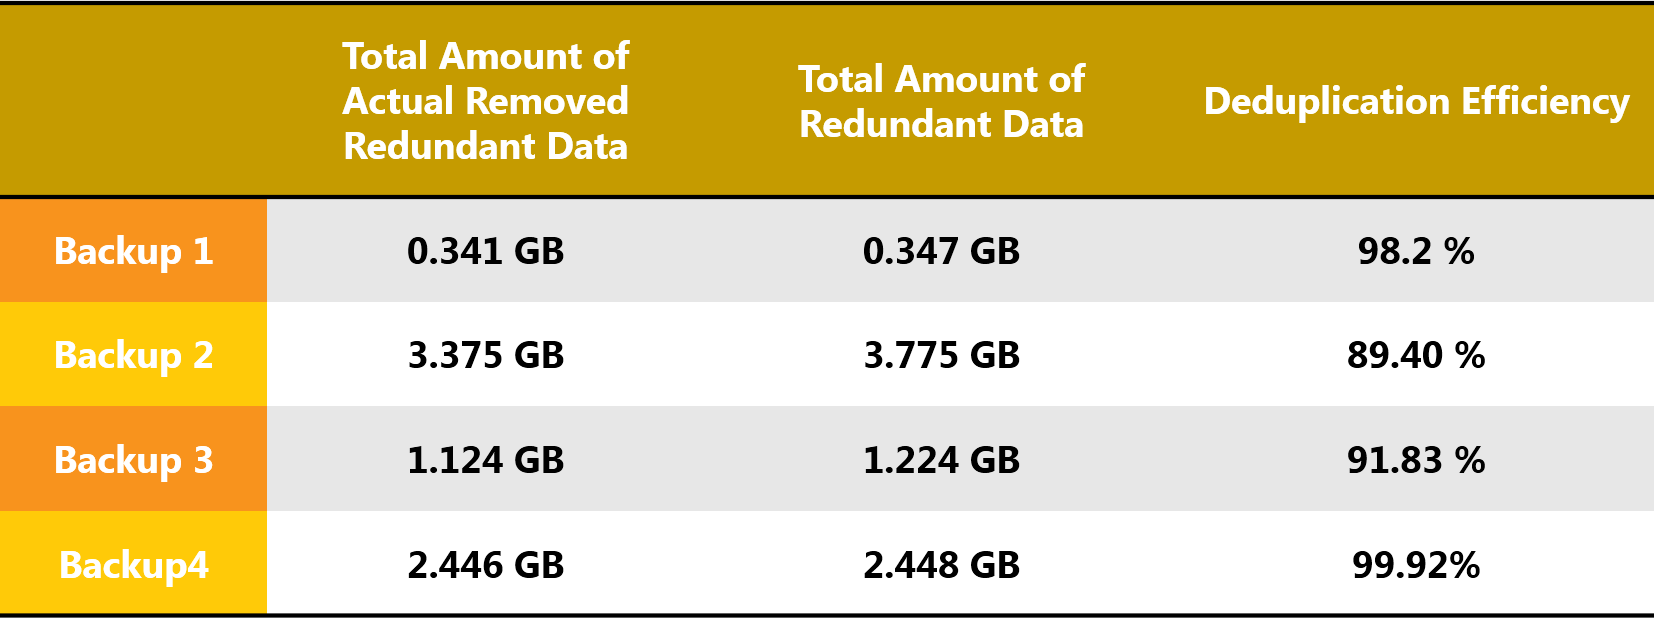
\includegraphics[height=1.5in, width=3in]{image5.png}
\caption{Dataset across five clients in four backup sessions. All numbers are in Gb.}
\end{figure}

\begin{figure}[!t]
\centering
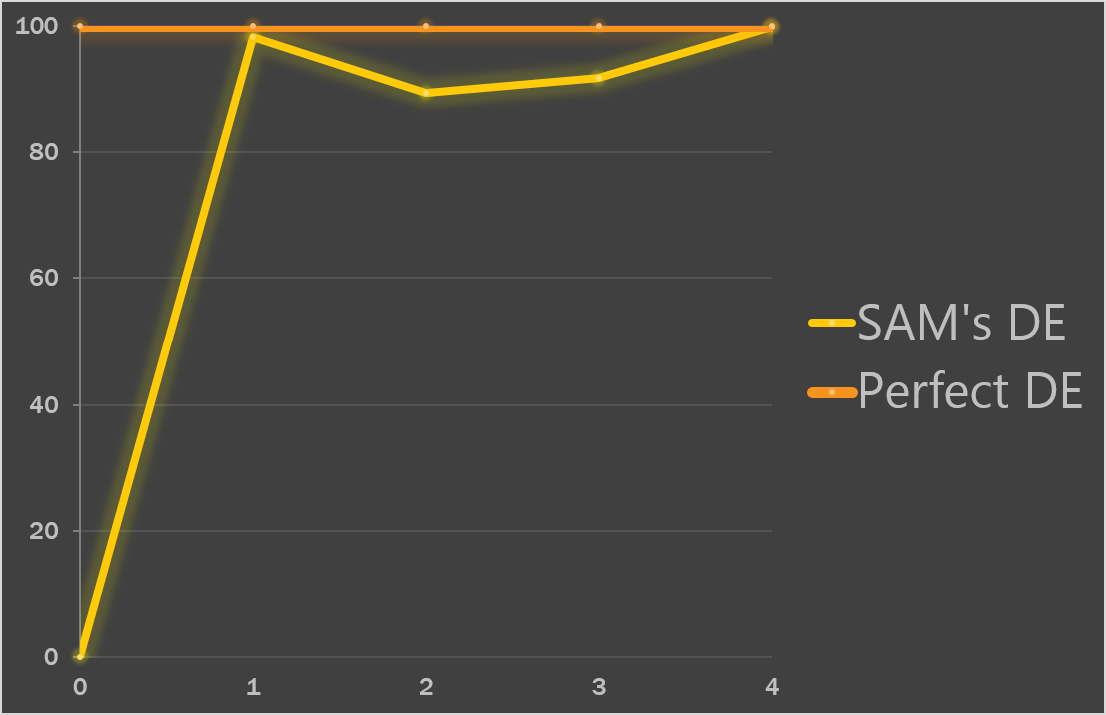
\includegraphics[height=1in, width=2in]{image7.png}
\caption{Deduplication Efficiency of SAM vs Maximum.}
\end{figure}

\begin{figure}[!t]
\centering
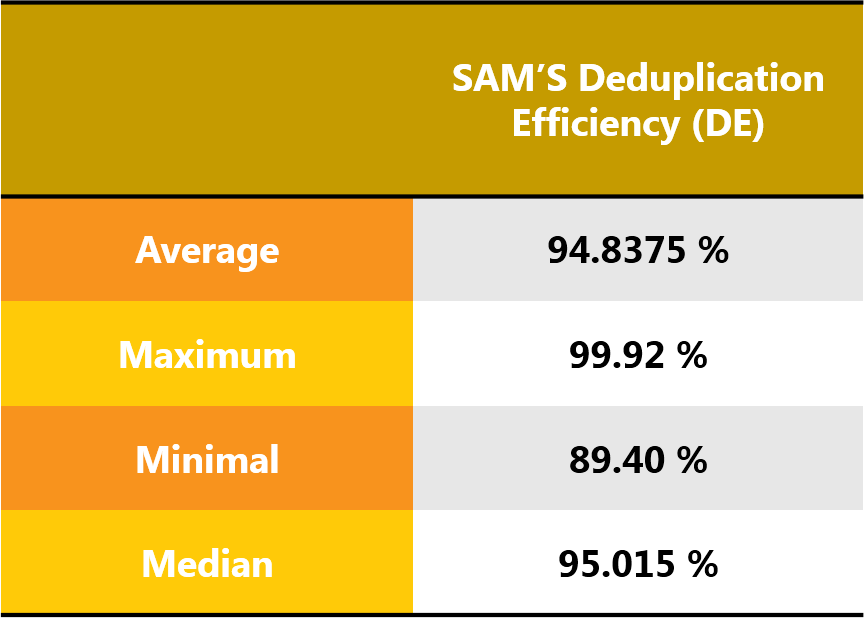
\includegraphics[height=1in, width=2in]{image8.png}
\caption{Deduplication Efficiency of SAM}
\end{figure}

\begin{figure}[!t]
\centering
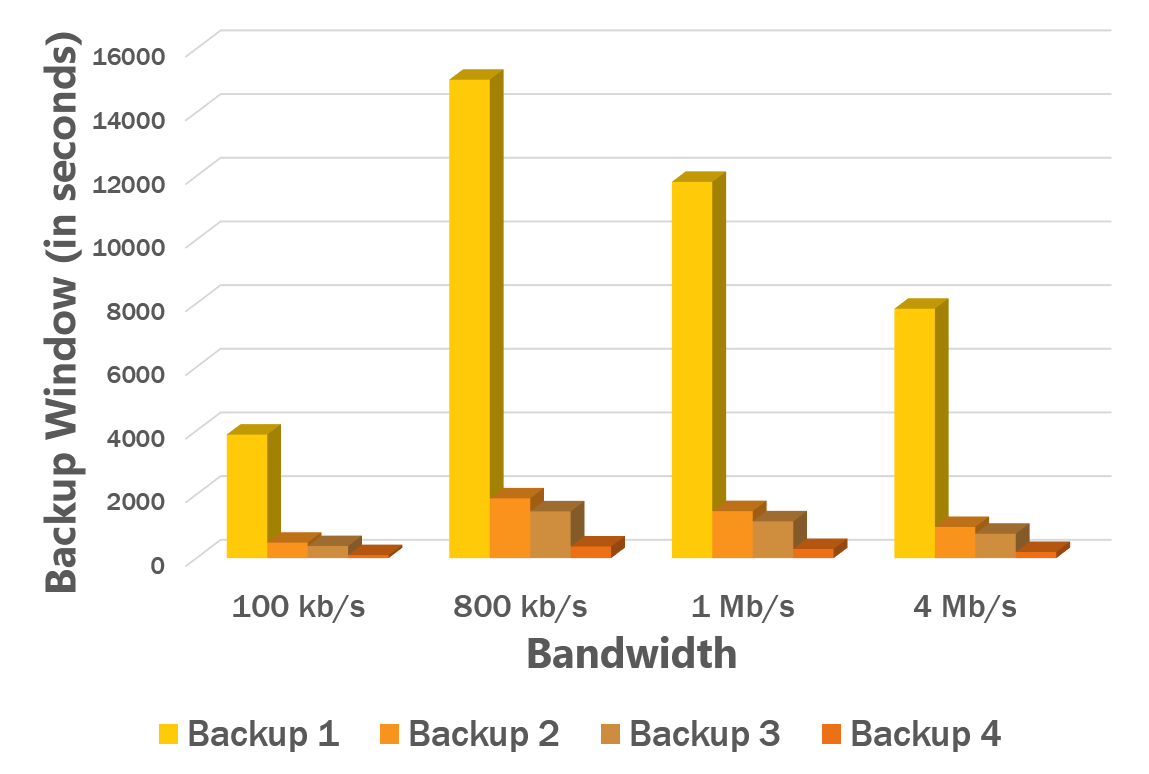
\includegraphics[height=1in, width=2in]{image9.png}
\caption{Backup Window of SAM}
\end{figure}


% can use a bibliography generated by BibTeX as a .bbl file
% BibTeX documentation can be easily obtained at:
% http://www.ctan.org/tex-archive/biblio/bibtex/contrib/doc/
% The IEEEtran BibTeX style support page is at:
% http://www.michaelshell.org/tex/ieeetran/bibtex/
%\bibliographystyle{IEEEtran}
% argument is your BibTeX string definitions and bibliography database(s)
%\bibliography{IEEEabrv,../bib/paper}
%
% <OR> manually copy in the resultant .bbl file
% set second argument of \begin to the number of references
% (used to reserve space for the reference number labels box)
\begin{thebibliography}{1}

\bibitem{malchik}
DeDu: Building a Deduplication Storage System over Cloud Computing
	
\bibitem{IEEE}
SAR: SSD Assisted Restore Optimization for Deduplication-based Storage Systems in the Cloud

\bibitem{IEEE}
SAM: A Semantic-Aware Multi-Tiered Source Deduplication Framework for Cloud Backup

\bibitem{IEEE}
AA-Dedupe: An Application-Aware Source Deduplication Approach for Cloud Backup Services in the Personal Computing Environment

\bibitem{IEEE}
Analysis of Data Fragments in Deduplication System

\bibitem{IEEE}
Reducing the De-Linearization of Data Placement to Improve Deduplication Performance

\bibitem{IEEE}
Chunk and Object Level Deduplication for Web Optimization: A Hybrid Approach

\bibitem{IEEE}
Detecting Duplicates over Sliding Windows with RAM-Efficient Detached Counting Bloom Filter Arrays

\bibitem{IEEE}
End-to-end Data Deduplication for the Mobile Web

\bibitem{IEEE}
Estimation of Deduplication Ratios in Large Data Sets

\bibitem{IEEE}
The Case for Content Search of VM Clouds

\bibitem{IEEE}
Semantic Data De-duplication for Archival Storage Systems

\bibitem{IEEE}
Large-Scale Deduplication with Constraints using Dedupalog

\bibitem{IEEE}
IM-Dedup: An Image Management System Based on Deduplication Applied in DWSNs

\end{thebibliography}

% biography section
% 
% If you have an EPS/PDF photo (graphicx package needed) extra braces are
% needed around the contents of the optional argument to biography to prevent
% the LaTeX parser from getting confused when it sees the complicated
% \includegraphics command within an optional argument. (You could create
% your own custom macro containing the \includegraphics command to make things
% simpler here.)
%\begin{biography}[{\includegraphics[width=1in,height=1.25in,clip,keepaspectratio]{mshell}}]{Michael Shell}
% or if you just want to reserve a space for a photo:

\end{IEEEbiography}

\vfill 

% insert where needed to balance the two columns on the last page with
% biographies
%\newpage

% You can push biographies down or up by placing
% a \vfill before or after them. The appropriate
% use of \vfill depends on what kind of text is
% on the last page and whether or not the columns
% are being equalized.

%\vfill

% Can be used to pull up biographies so that the bottom of the last one
% is flush with the other column.
%\enlargethispage{-5in}



% that's all folks
\end{document}